\documentclass[11pt]{article}

\textwidth 16cm \textheight 23cm \evensidemargin 0cm
\oddsidemargin 0cm \topmargin -2cm
\parindent 0pt
\parskip \medskipamount


\usepackage[dutch]{babel}
\usepackage{amssymb}
\usepackage{amsmath}
\usepackage[utf8]{inputenc}
\usepackage[normalem]{ulem} % strikethrough normal text with \sout{text}
\usepackage{cancel} % strikethrough in math mode with \cancel{text}
\usepackage{hyperref}

\usepackage{subfig}
\usepackage{wrapfig}
\usepackage{graphicx}

\usepackage[table]{xcolor}

\usepackage{pgf,tikz}
\usetikzlibrary{arrows}

\usepackage{color}
\newcommand{\todo}[1]{\textcolor{red}{\##1\#}}
\newcommand{\question}[1]{\textcolor{blue}{\##1\#}}

\newcommand{\vraag}[2]{\begin{itemize}\item #1 \vspace{#2}\end{itemize}}

\newcommand{\degree}{\ensuremath{^\circ}}

\graphicspath{{../figuren/}}

\begin{document}

\section{Iets statistisch onderzoeken}

We wensen een statistisch onderzoek uit te voeren. Wat wil dit nu zeggen? Wel, {\it onderzoeken} is iets nauwkeurig nazien of nagaan. Een voorbeeld zou kunnen zijn: {\it Tot hoe laat mogen jongeren in het weekend uitgaan?}. De vraag die bij een onderzoek hoort noemen we de {\bf onderzoeksvraag}. Een {\it statistisch onderzoek} is dan een onderzoek die verloopt volgens de statistiek. De {\bf statistiek} is de wetenschap van het waarnemen van verschijnselen en het weergeven van de uitkomsten in getallen en figuren. In het vorig voorbeeld wil dit zeggen dat we {\it waarnemen} bij anderen tot hoe laat deze uitgaan. Deze waarnemingen gaan we dan zo goed mogelijk {\it weergeven}, dit met getallen of figuren.

Een onderzoek kan in vier stappen verlopen:
\begin{enumerate}
  \item Wat wil je weten? Hoe ga je meten?
  \item Op speurtocht gaan in de dataset.
  \item Wat heb je gevonden? Hoe ver kan je gaan in je conclusie?
  \item Kernachtig samenvatten van onderzoek.
\end{enumerate}

Wat de stappen inhouden zullen we zien aan de hand van een aantal voorbeelden.

\section{Statistisch onderzoek naar de kleuren van M\&M-snoepjes}

\subsection{De onderzoeksvraag}

\begin{wrapfigure}{r}{0.4\textwidth}
  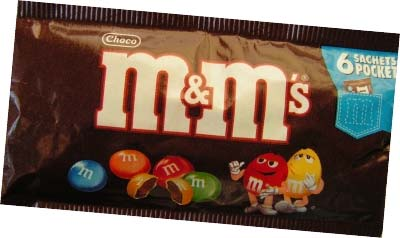
\includegraphics[width=0.4\textwidth]{MenM-verpakking.png}
\end{wrapfigure}

Iedereen kent wel M\&M’s, de chocoladesnoepjes met de felgekleurde suikerjasjes. De fabrikant van
M\&M’s stopt verschillende kleuren snoepjes in één verpakking.

Heb je enig idee welke kleuren allemaal voorkomen bij M\&M’s?
Komt elke kleur evenveel voor? Dat ga je nu onderzoeken.

Je hebt hier al een eerste probleem. Wat wil je eigenlijk
onderzoeken? Wil je iets zeggen over de kleuren in je eigen zakje
M\&M”s of wil je iets zeggen over de kleuren van alle M\&M-
snoepjes die door de fabrikant gemaakt worden? Dat zijn nogal
verschillende vragen!

\subsection{Een dataset maken}

Om goed het onderscheid te maken tussen “alle M\&M’s” en “de snoepjes in jouw zakje M\&M’s”
gebruikt de statistiek twee verschillende woorden. Je spreekt over {\bf populatie} als je “de totale
verzameling” bedoelt (dus alle M\&M-snoepjes). Meestal heb je geen tijd of geld om een volledige
populatie te onderzoeken en daarom bekijk je enkel een klein deeltje van die populatie. Zo’n deeltje
van een populatie wordt in de statistiek een {\bf steekproef} genoemd. De snoepjes die in je zakje
M\&M’s zitten, zijn een heel klein deeltje van alle M\&M’s. Jouw snoepjes zijn dus een steekproef uit
de totale populatie van alle M\&M’s.

Je steekproef bestaat uit dingen die je zelf hebt verzameld, die je dus zelf kan zien en beschrijven
(met getallen en grafieken). Hoe je dat doet, dat ga je in dit onderzoek leren. Maar misschien wil je
daarna ook iets zeggen over alle M\&M’s. Misschien zijn de blauwe snoepjes in jouw zakje in de
meerderheid. Zou je dan kunnen zeggen dat bij alle M\&M’s de blauwe snoepjes het meest
voorkomen? (Let op! Misschien heeft een andere leerling meer rode snoepjes).

Iets zeggen over de totale populatie als je enkel de steekproef ziet, dat is helemaal niet eenvoudig.
Statistiek kan je hierbij helpen. Een eerste hulp die de statistiek je biedt, gaat over de manier waarop
je een steekproef moet trekken. De raadgeving die je hier krijgt, had je waarschijnlijk nooit
verwacht. Om een goede steekproef te trekken, moet je je laten leiden door ... het toeval!

Je laten leiden door het toeval, dat is gemakkelijker gezegd dan gedaan. M\&M's worden gemaakt in verschillende
kleuren volgens een verhouding die door de fabrikant is vastgelegd. Die snoepjes komen terecht in
een reuzegrote container waar ze grondig door elkaar worden gemengd. Daarna wordt uit die
container lukraak een schep snoepjes genomen en die snoepjes worden in een zakje verpakt. Dat
gebeurt natuurlijk allemaal volautomatisch en in superhygiënische omstandigheden.

Die enorme container, waarin miljoenen M\&M’s zitten, kan je beschouwen als een goed model voor
de hele populatie. Een goede steekproef trek je dan als volgt: “goed mengen en dan lukraak trekken”.
Deze manier van werken krijgt in de statistiek de naam “{\bf enkelvoudige aselecte steekproef}”. Het
aantal elementen in je steekproef (het aantal getrokken snoepjes) noteer je door de letter “$n$” (dat
noem je de {\bf steekproefgrootte}).

De informatie in je steekproef ga je nu op een overzichtelijke manier opschrijven in een tabel. Zo krijg je de
{\bf gegevensverzameling of dataset}. In zulk een tabel staan op de rijen de {\bf elementen}, deze zijn de objecten die in een statistische studie worden onderzocht. In ons geval heb je voor elke M\&M één rij. In de kolommen staan de {\bf veranderlijken}, elke veranderlijke is één welbepaalde eigenschap die je opmeet. Zo kunnen we voor elke M\&M de kleur noteren.

\vraag{Maak een tabel waarin je de gegevens zal opschrijven. Als je afkortingen gebruikt, schrijf dan ook op wat die afkortingen betekenen.}{10cm}

\subsection{De dataset: getallen en context}
Bij de dataset die je pas hebt opgesteld is er één kolom waarin je de kleur van de snoepjes hebt
geschreven. Je hebt hier te maken met een “eigenschap van snoepjes”, namelijk “hun kleur”. Dit is
een “veranderlijke” die jij hebt opgemeten. Deze veranderlijke heeft hier de waarden: rood, groen,
blauw, bruin, en geel.
Op kleuren kan je geen zinvolle wiskundige bewerkingen uitvoeren zoals optellen of
vermenigvuldigen. Daarom noemt men de veranderlijke “kleur” een {\bf kwalitatieve veranderlijke}.

Er is een belangrijk onderscheid tussen de naam van een veranderlijke en de
verschillende waarden van die veranderlijke.
In dit geval is “kleur” de {\bf naam} van de veranderlijke en “rood, groen, blauw,
...” zijn de mogelijke {\bf waarden}.

\subsection{Op speurtocht in de dataset}

Je dataset is de basis voor al je verder onderzoek. De dataset, samen met de beschrijving van hoe je
hem hebt opgemeten, moet je nauwkeurig bewaren.

\subsubsection{Een frequentietabel opstellen}

\vraag{Gebruik je dataset om een frequentietabel op te stellen. Doe dat zoals hieronder aangegeven.}{0cm}

In de eerste kolom schrijf je de kleuren en in de tweede kolom schrijf je hoeveel snoepjes er van die
kleur zijn. Dit aantal heet de {\bf frequentie} van die kleur. Een tabel die je op deze manier opstelt, heet
een {\bf frequentietabel}. Zorg ervoor dat je elke kolom een juiste naam geeft: deze naam schrijf je
bovenaan de kolom.

\begin{center}
  \begin{tabular}{|p{2cm}|p{2cm}|p{2cm}|}
    \hline
    &&\vspace*{0pt}\\
    \hline
    &&\vspace*{0pt}\\
    \hline
    &&\vspace*{0pt}\\
    \hline
    &&\vspace*{0pt}\\
    \hline
    &&\vspace*{0pt}\\
    \hline
    &&\vspace*{0pt}\\
    \hline
    &&\vspace*{0pt}\\
    \hline
  \end{tabular}
\end{center}
\vspace{1cm}

\vraag{Hoe kan je de steekproefgrootte snel berekenen met behulp van de frequentietabel?}{4cm}

We gaan nu een derde kolom aan de frequentietabel toevoegen. In die kolom komt, per kleur, {\bf de
relatieve frequentie}. De relatieve frequentie is niets anders dan de frequentie gedeeld door het totale
aantal $n$ . Je kan dit getal ook in percent uitdrukken. Als je voor “geel” een relatieve frequentie van
0.16 vindt, dan kan je dat ook schrijven als 16\%. Hierbij rond je af op één eenheid. In woorden zeg
je dat 16\% van jouw onderzochte snoepjes geel is.

Om zoveel mogelijk van je tijd te kunnen besteden aan nadenken en
discussiëren, ga je zo weinig mogelijk tijd besteden aan slaafse
berekeningen. We gebruiken software op een verstandige manier. Zo leer je ook
hoe elk “echt” statistisch onderzoek verloopt.

We starten {\it Geogebra} en kiezen 'Beeld-Rekenblad' om het rekenblad te tonen. Het algebravenster en het tekenblad mogen verborgen worden. De eerste kolom vullen we met de frequenties. Als je bijvoorbeeld $13$ rode, $9$ groene, $8$ gele, $7$ oranje, $7$ bruine en $6$ blauwe snoepjes had, dan ga je als volgt te werk. In de eerste {\bf cell} rechtsboven vul je 13 in. Deze cell noemt A1. In de cell eronder vul je $9$ in. Je gaat zo verder tot aan cell A6. De cellen A1 tot aan A6 noteren we met A1:A6 en deze wordt een {\bf lijst} genoemd.

In de tweede kolom, in cell B1, vul je 
$$
=A1 / \mbox{Som}[A1:A6]
$$
in. Het gelijk aan teken '=' maakt aan Geogebra duidelijk dat wat volgt berekend moet worden. Geogebra zal in dit geval de waarde in de cell A1 delen door de som van de cellen in de lijst A1:A6. Nu doen we dit ook voor de andere cellen in de tweede kolom, waarbij dan op de juiste plaats A1 vervangen wordt.

\begin{center}
  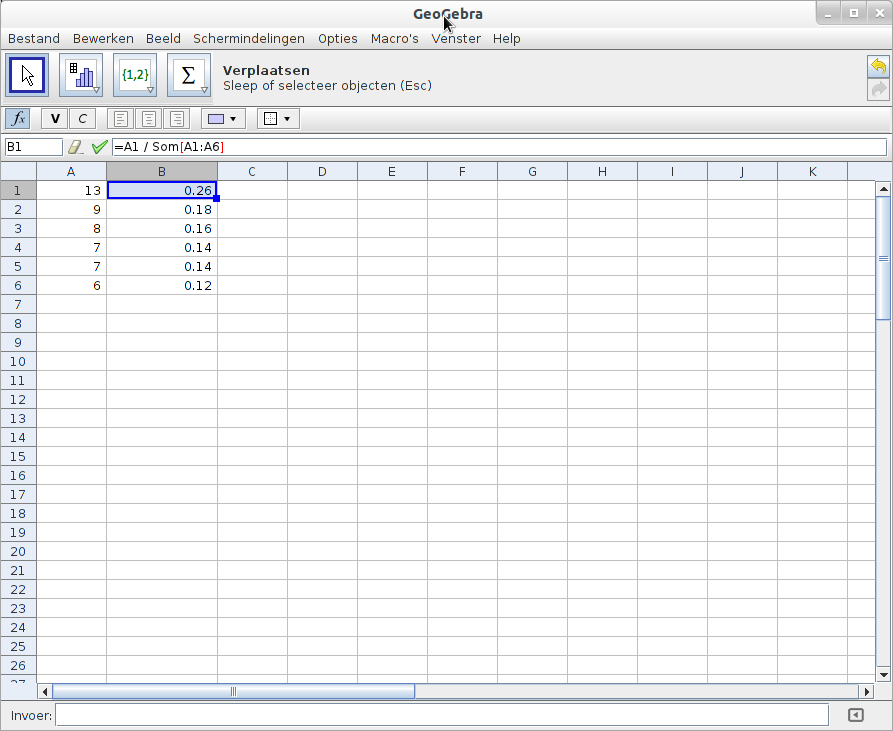
\includegraphics[width=14cm]{gg-relatieve_frequentie.png}
\end{center}

\vraag{Voeg aan je tabel een derde kolom toe met naam “relatieve frequentie” en schrijf daarin de
resultaten die in Geogebra staan (in percent). Tel de percenten bij elkaar op. Hoeveel heb je?
}{3cm}

Soms heb je frequenties nodig, in andere gevallen gebruik je relatieve frequenties. Als je aantallen
bestudeert, dan werk je met frequenties. Als je percentages gebruikt om twee onderzoeken met
elkaar te vergelijken, dan werk je met relatieve frequenties.

{\bf Voorbeeld}\\
Om te weten of je genoeg rode snoepjes hebt om er eentje te kunnen geven aan elk van je 10
vrienden, dan kijk je naar de frequentie.
Als je de kleurensamenstelling van een grote en een kleine zak M\&M’s wil vergelijken, dan zal je
met percentages werken en dus relatieve frequenties gebruiken.



\subsection{Figuren tekenen}

\begin{wrapfigure}{r}{0.3\textwidth}
  \vspace{-0.5cm}
  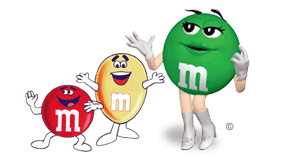
\includegraphics[width=0.3\textwidth]{MenM-fun.png}
\end{wrapfigure}

Veruit het meest belangrijke onderdeel bij de studie van een
dataset is kijken naar figuren. Dit is niet eenvoudig en je
moet stapsgewijs leren waar je allemaal moet op letten.
Zodra je dit wat kent, kan je uit een figuur heel veel
informatie halen. Maar je moet natuurlijk eerst weten welke
figuur je moet maken en hoe je die moet tekenen.

\subsection{Een staafdiagram}

Je hebt in dit onderzoek een nominaal kwalitatieve veranderlijke opgemeten. Voor dit soort
veranderlijken is het {\bf staafdiagram} de basisfiguur.

\begin{wrapfigure}{r}{0.4\textwidth}
  \vspace{-0.5cm}
  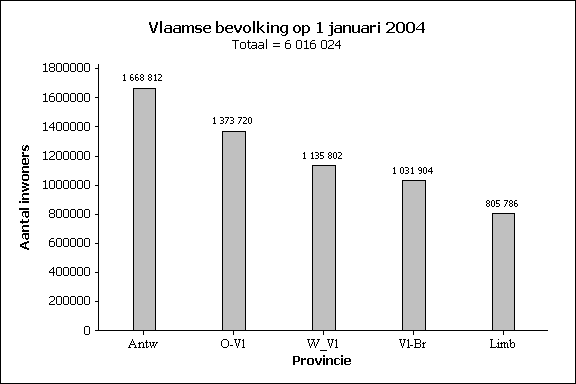
\includegraphics[width=0.4\textwidth]{vlaamse_bevolking.png}
\end{wrapfigure}
Als voorbeeld zie je hier een staafdiagram
van de Vlaamse bevolking per provincie. De
informatie die hier wordt weergegeven, kan
je vinden in het boekje “Vlaanderen in
cijfers” op de website:
\url{http://aps.vlaanderen.be/statistiek/publicaties/pdf/vic/vic2005.pdf}.
De namen van de provincies zijn afgekort als:
Antw = Antwerpen,
O-Vl = Oost-Vlaanderen,
W-Vl = West-Vlaanderen,
Vl-Br = Vlaams - Brabant,
Limb = Limburg.



\end{document}























